% Source : http://forum.mathematex.net/latex-f6/tableaux-de-proportionnalite-t3752.html?hilit=tableau

\documentclass[]{article} 
	\usepackage{tikz,fullpage}
	\usetikzlibrary{arrows}


\begin{document}

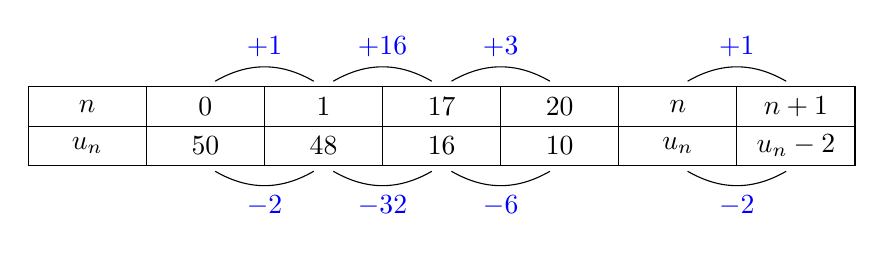
\begin{tikzpicture}
	\tikzstyle{every to}=[->,blue,thin,>=stealth']
	\newcounter{numcase}\setcounter{numcase}{0}
	\foreach \x/\xtext/\ytext in {0/n/u_{n},1.5/0/50,3/1/48,4.5/17/16,6/20/10,7.5/n/u_{n},9/n+1/u_{n}-2} { %
		\stepcounter{numcase}
		\draw (\x,0.5) +(-0.75,-0.25) rectangle ++(0.75,0.25) ;
		\draw (\x,0)   +(-0.75,-0.25) rectangle ++(0.75,0.25);
		\node[]  at (\x,0.5) {$\xtext$};
		\node[]  at (\x,0)   {$\ytext$};
		\node[] (x_\thenumcase)  at (\x,0.75) {};
		\node[] (y_\thenumcase) at (\x,-0.25) {};%
	}
	\draw (x_2) to [bend left]  node[above]{$+1$} (x_3);
	\draw (y_2) to [bend right] node[below]{$-2$} (y_3);
	\draw (x_3) to [bend left]  node[above]{$+16$} (x_4);
	\draw (y_3) to [bend right] node[below]{$-32$} (y_4);
	\draw (x_4) to [bend left]  node[above]{$+3$} (x_5);
	\draw (y_4) to [bend right] node[below]{$-6$} (y_5);
	\draw (x_6) to [bend left]  node[above]{$+1$} (x_7);
	\draw (y_6) to [bend right] node[below]{$-2$} (y_7);
\end{tikzpicture}

\end{document}
